Grâce à l'introduction du support des fichiers glTF ou plus précisément des fichiers glb dans la spécification 3D Tiles 1.1, il est devenu beaucoup plus facile de générer des fichiers 3D comparé à l'ancien système. Ici, j'utilise la librairie \href{https://github.com/javagl/JglTF}{jglTF}\footnote{https://github.com/javagl/JglT} et la librairie \href{https://locationtech.github.io/jts/}{JTS}\footnote{https://locationtech.github.io/jts/} pour créer les nodes, les meshes, les materials et les textures des bâtiments. Toute la ligique concernant la création des fichiers glTF se trouve dans la classe \texttt{GltfBuilder}\footnote{baremaps-core/src/main/java/org/apache/baremaps/tdtiles/GltfBuilder.java}.

\subsection{Système de compression des géométries des bâtiments}

Comme vu à la section \ref{sec:lod}, il est nécessaire de pouvoir fournir plusieurs niveaux de détails en fonction du niveau de la tuile. Pour cela, j'ai implémenté un système de compression des géométries des bâtiments. Ce système se base sur les \texttt{levels} des tuiles discutés à la section \ref{sec:implicit-tiling}. Plus le \texttt{level} est élevé, plus les bâtiments sont proches de la caméra et donc plus les bâtiments doivent être détaillés. Pour effectuer la compression, j'utilise la class \texttt{DouglasPeuckerSimplifier} qui permet de simplifier une géométrie en fusionnant les points les plus proches d'une géométrie.

En fonction du \texttt{level} de leur tuile, les bâtiments subissent jusqu'à 3 niveau de compression :

\begin{itemize}
    \item \texttt{level} 0 : Les bâtiments sont affichés avec toutes les géométries.
    \item \texttt{level} 1 : Les bâtiments sont affichés avec une géométrie légèrement simplifiée.
    \item \texttt{level} 2 : Les bâtiments sont affichés avec une géométrie très simplifiée.
    \item \texttt{level} 3 : Les bâtiments sont affichés avec une géométrie très simplifiée uniquement si ils ont des caractéristiques spécifiques enregistrées dans la base de données OSM.
\end{itemize}

Pour visualiser les différences entre les niveaux de compression, je vous invite à regarder la figure \ref{fig:lods-colors} où chaque niveau de détail est simbolisé par une couleur :

\begin{itemize}
    \item \texttt{level} 0 : rouge
    \item \texttt{level} 1 : vert
    \item \texttt{level} 2 : bleu
    \item \texttt{level} 3 : blanc
\end{itemize}

% TODO: outdated image

\begin{figure}[H]
    \centering
    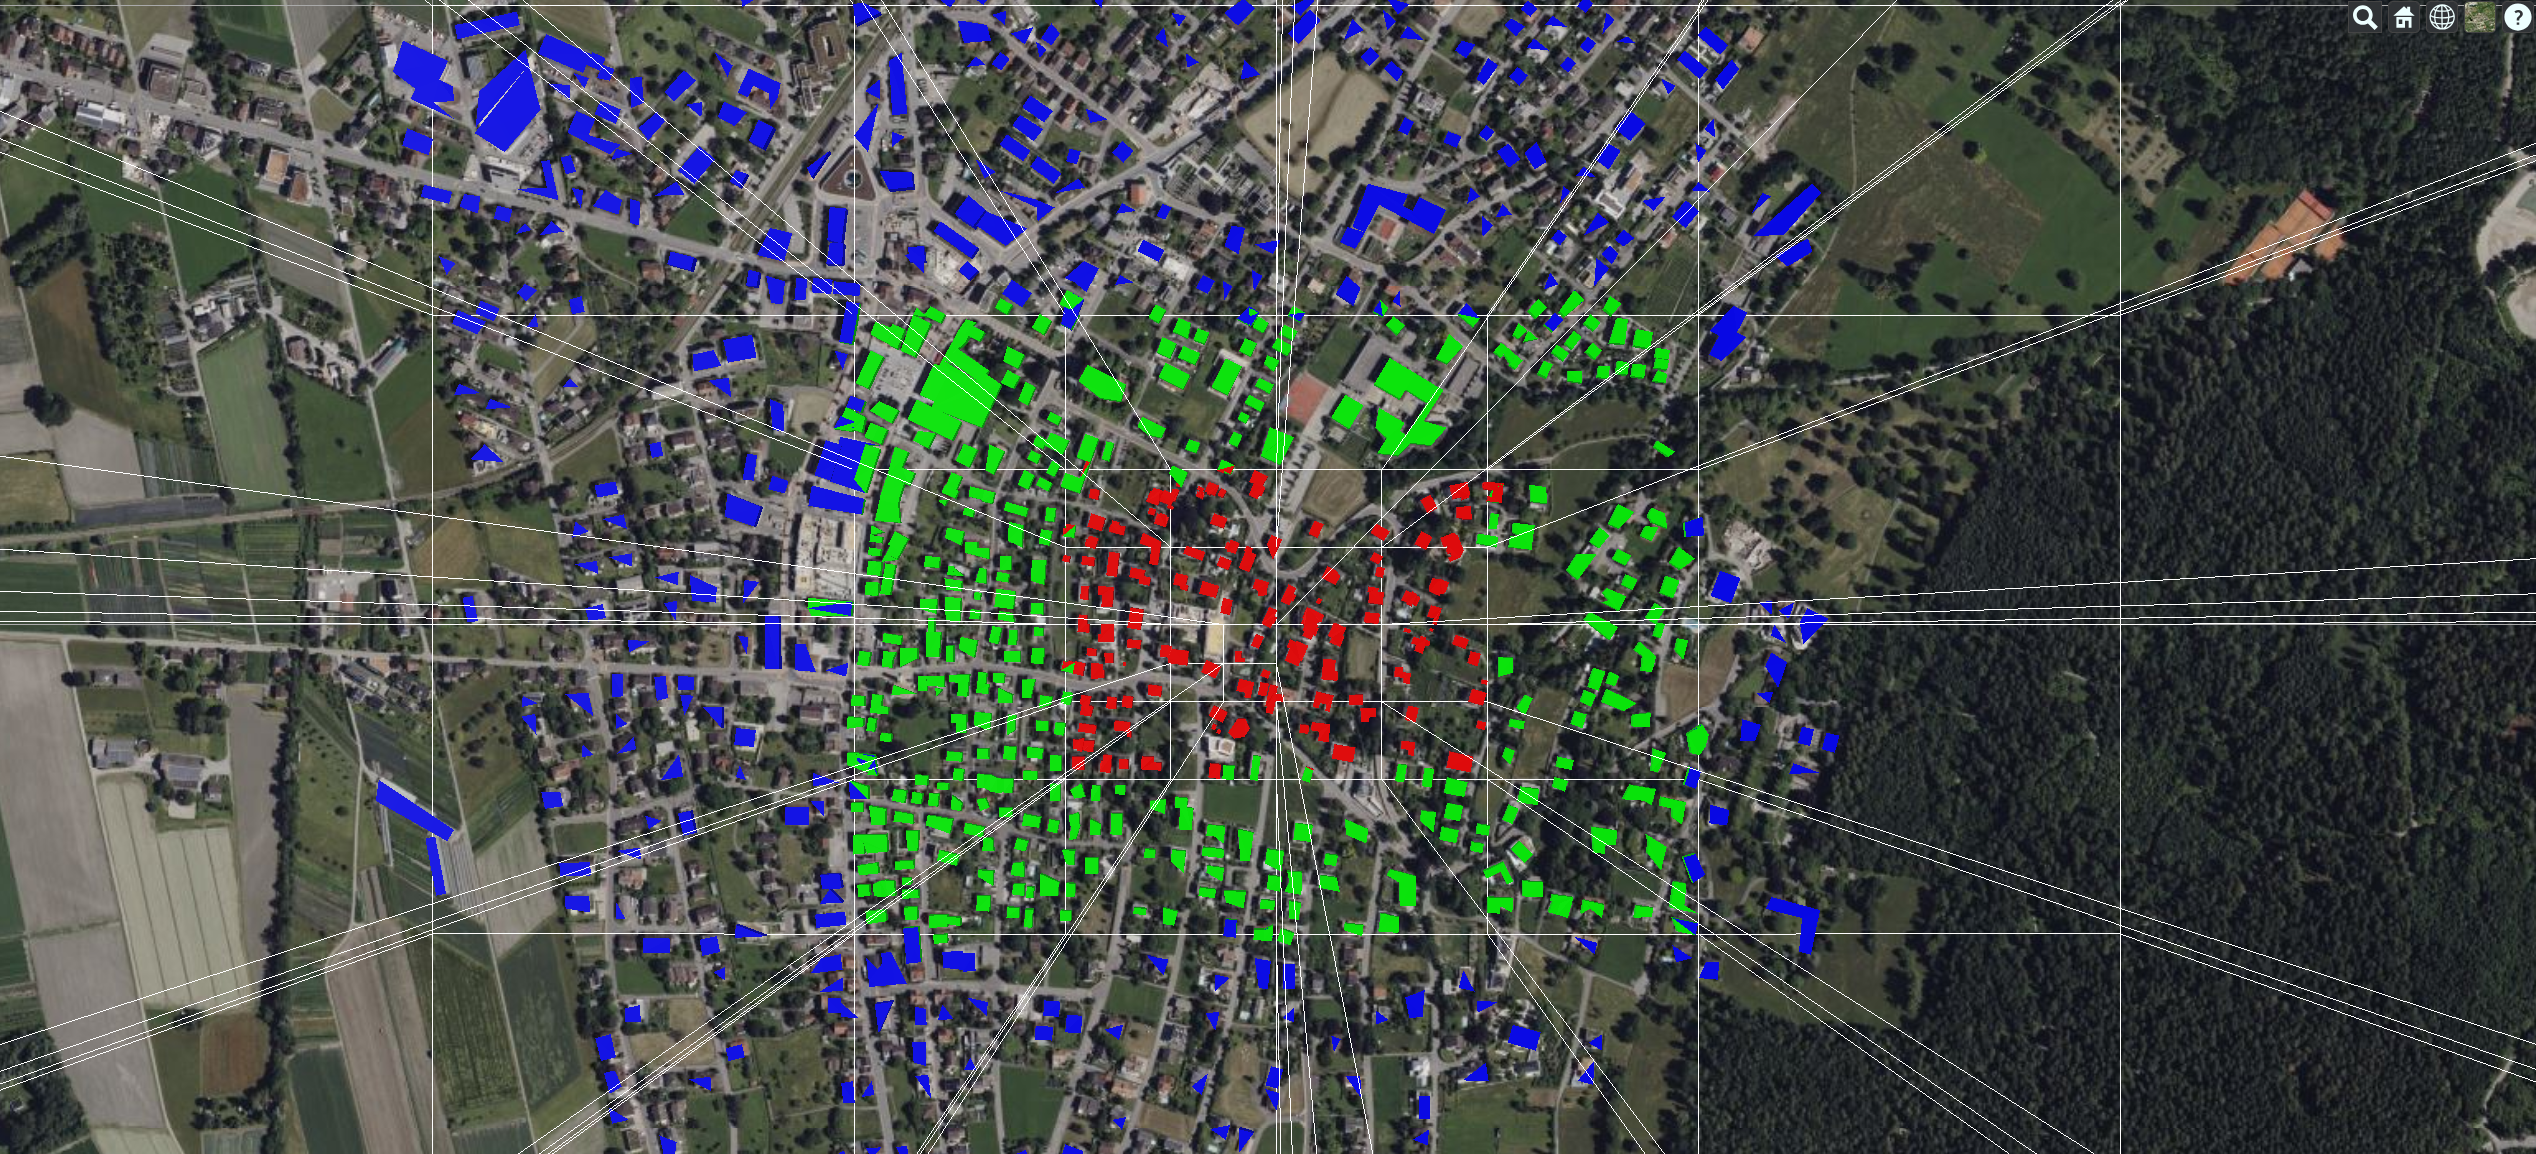
\includegraphics[width=1\textwidth]{assets/figures/s2-Cells_and_implicit_auto_LODs.png}
    \caption{Calcul du SSE \cite{3d-tiles-specification}}
    \label{fig:lods-colors}
\end{figure}

Faire ainsi permet de réduire drastiquement le temps passé à générer ces bâtiments tout en gardant une qualité d'affichage correcte.

\subsection{Géométries des bâtiments}

Avec le niveau de compression ainsi que la \texttt{Geometry}\footnote{org.locationtech.jts.geom.Geometry}, qui nous sert à déterminer le polygone au sol du bâtiment, nous pouvons extruder le bâtiment en 3D. Cependant une \texttt{Geometry} ne contient qu'une liste de points et il faut une liste de triangles pour pouvoir modéliser le bâtiment en 3D. Pour cela, la méthode \texttt{DelaunayTriangulationBuilder}\footnote{org.locationtech.jts.triangulate.DelaunayTriangulationBuilder} était utilisée. Le problème était que la \href{https://en.wikipedia.org/wiki/Delaunay_triangulation}{\textit{Delaunay triangulation}}\footnote{https://en.wikipedia.org/wiki/Delaunay\_triangulation} ne fonctionne pas avec des polygones concaves. Une version complémentaire de cette méthode est la \href{https://en.wikipedia.org/wiki/Constrained_Delaunay_triangulation}{\textit{Constrained Delaunay triangulation}}\footnote{https://en.wikipedia.org/wiki/Constrained\_Delaunay\_triangulation} qui fonctionne avec des polygones concaves en définissant des segments comme bords du polygone. Cette version de l'algorithme est aussi disponible dans la librairie \texttt{JTS} mais elle propose aussi la classe \href{https://locationtech.github.io/jts/javadoc/org/locationtech/jts/triangulate/polygon/PolygonTriangulator.html}{\texttt{PolygonTriangulator}}\footnote{https://locationtech.github.io/jts/javadoc/org/locationtech/jts/triangulate/polygon/PolygonTriangulator.html} qui permet aussi de faire une triangulation de polygones concaves de manière moins optimisée mais plus rapide que la \textit{Constrained Delaunay triangulation}. C'est donc cette classe que j'ai utilisée pour trianguler les bâtiments.

Grâce à cette nouvelle triangulation, il est possible de modéliser les bâtiments en 3D correctement, même ceux comprenant des cours intérieures ou des trous dans leur structure.

La classe \texttt{DelaunayTriangulationBuilder} comportait cependant un paramètre \texttt{tolerance} qui permettait de définir la distance minimale entre deux points afin d'optimiser le coût de la triangulation. Cette possibilité n'est pas disponible dans la classe \texttt{PolygonTriangulator}, néanmoins j'implémente une alternative dans le chapitre suivant.

\subsection{Hauteur des bâtiments}

Le calcul de la hauteur des bâtiments doit se faire en fonction de la \href{https://wiki.openstreetmap.org/wiki/Simple_3D_Buildings}{définition}\footnote{https://wiki.openstreetmap.org/wiki/Simple\_3D\_Buildings} des bâtiments par OSM. Si aucun tags ne donne la hauteur du bâtiment, il aura par défaut une hauteur de 10 mètres. Sinon, la hauteur du bâtiment est calculée en fonction des tags \texttt{height}, \texttt{building:levels}, \texttt{building:min\_level}, \texttt{roof:height} et \texttt{roof:levels} :

\begin{itemize}
    \item On commence avec une hauteur de bâtiment de 0 mètres.
    \item Si aucun tag n'est présent,
          \begin{itemize}
              \item La hauteur du bâtiment est de 10 mètres.
          \end{itemize}
    \item Sinon, si le tag \texttt{height} est présent,
          \begin{itemize}
              \item La hauteur du bâtiment est égale à la valeur du tag \texttt{height}.
              \item Si le tag \texttt{roof:height} est présent,
                    \begin{itemize}
                        \item La hauteur du toit \texttt{roof:height} doit être soustraite de la hauteur du bâtiment
                    \end{itemize}
          \end{itemize}
    \item Sinon,
          \begin{itemize}
              \item Si le tag \texttt{building:levels} est présent,
                    \begin{itemize}
                        \item La hauteur du bâtiment est égale à la valeur du tag \texttt{building:levels} multipliée par 3 mètres.
                    \end{itemize}
              \item Si le tag \texttt{roof:levels} est présent,
                    \begin{itemize}
                        \item La hauteur du toit \texttt{roof:levels} multipliée par 3 mètres doit être additionnée à la hauteur du bâtiment.
                    \end{itemize}
              \item Si le tag \texttt{building:min\_level} est présent,
                    \begin{itemize}
                        \item La hauteur du vide en dessous du bâtiment est égale à la valeur du tag \texttt{building:min\_level} multipliée par 3 mètres.
                    \end{itemize}
          \end{itemize}
\end{itemize}

La hauteur connue, on peut la transmettre à la classe \texttt{GltfBuilder} pour donner la hauteur au bâtiment lors de sa modélisation.

\subsection{glTF par bâtiment ou par tuile}

Quand on pense aux manière de générer les fichiers 3D, il est facile de concevoir que deux méthodes sont possibles : générer un fichier glTF par bâtiment ou générer un fichier glTF par tuile. La première méthode nous permettrait de générer des features par bâtiment glTF, ce qui rendrait l'utilisation de metadata très intéressante.

Plus intéressant encore, générer ces fichiers 3D par bâtiment nous pousserai fortement à tenir une liste de bâtiments se trouvant dans chaque tuile. En faisant ainsi, il serait possible de prévenir le placement d'un même bâtiment dans plusieurs tuiles. Souvent, un bâtiment se trouve à cheval sur plusieurs tuiles et il est donc nécessaire de le placer dans plusieurs fichiers glTF quand on génère un fichier par tuile.

Pour pouvoir générer un fichier glTF par bâtiment, il faut utiliser le concept de \textit{Multiple Content} introduit dans la version 1.1 de la spécification 3D Tiles \cite{3d-tiles-reference-card-v1_1}. Pour utiliser cela, il faut remplacer le champ \texttt{content} de chaque tuile par un champ \texttt{contents} qui sera une liste de plusieurs \texttt{content}. Chaque \texttt{content} contiendra un \texttt{uri} qui pointera vers le fichier glTF du bâtiment.

Cependant, un problème survient si l'on utilise en même temps l'implicit tiling lors de la génération des \textit{Subtrees}. Ces Subtrees, définits plus en profondeur dans leur chapitre dédié, nécessitent une liste de disponibilité (\autoref{sec:availability-class}) \textbf{par content}. En d'autres termes, si une tuile contient $X$ bâtiments, il faudra $X$ listes de disponibilité sur la tuile. Sur chacune de ces listes, une seule valeur sera à \texttt{true}, la valeur correspondant à l'index de la tuile sur laquelle le bâtiment se trouve. Cela rend donc la génération des Subtrees beaucoup plus complexe et énormément plus volumineuse. Pour plus de précisions sur le pourquoi de cette complexité, je vous invite à lire le chapitre dédié aux Subtrees.